\chapter{Présentation de la problématique}
    \label{Chapitre 3}
    \section{Présentation du sujet}
    Le projet avec le laboratoire \textit{Biologie} de l'\textit{Université des Antilles}, concerne l'analyse de déplacement de \textbf{Gerridés}.

    Le but étant de déterminer leur préférence entre différentes zones marquées par des odeurs, en environnement contrôlé.

    % \vspace{0.5cm}

    \section{Présentation de l'aspect biologiste}
    Les \textbf{Gerridés} sont une famille d'insectes de l'ordre des Hémiptères et du sous-ordre des Hétéroptères c'est-à-dire des punaises.
    \begin{figure}[ht]
        \centering
        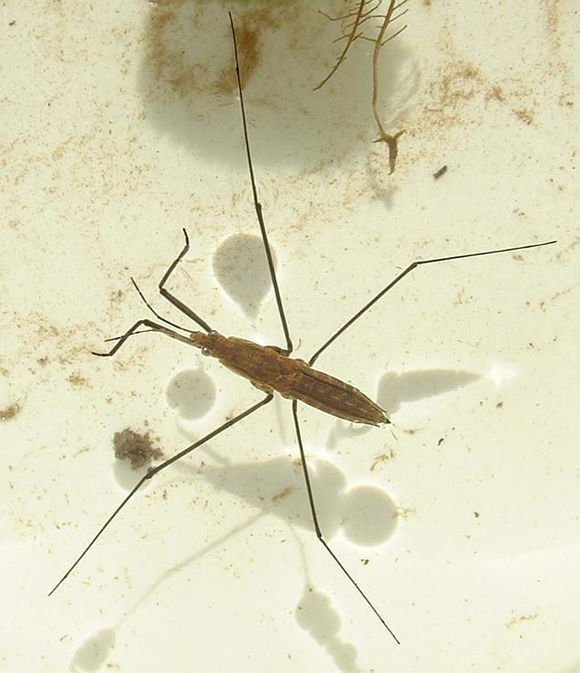
\includegraphics[scale=0.15]{gerrides.jpg}
        \caption{Gérridés}        
    \end{figure}

    \vspace{0.1cm}

    
    Les membres de cette famille sont communément appelés araignées d’eau, mais ce sont des insectes, on ne peut donc pas parler d'araignées. Cette appellation vient sans doute du fait de leurs longues pattes. Leur capacité à se déplacer sur l'eau leur vaut aussi le nom de patineurs de l'eau.

    Dans un environnement contrôlé, on place deux zones avec différentes odeurs (aliments) et on observe où les \textbf{Gerridés} préfèrent se déplacer. Afin de faciliter l'enregistrement de l'expérience, il est nécessaire d'avoir un système adéquat de capture vidéo.
     
    \subsection{Positionnement du travail dans le projet}
        Les biologistes accrochaient une GoPro au-dessus du bac et ensuite devaient la retirer afin de pouvoir récupérer les données enregistrées. Ce dispositif était fonctionnel et leur permettait de réaliser des captures vidéo mais il leur fallait placer le bac dans le champ de vision de la GoPro a chaque fois qu'ils voulaient faire une capture.



        \vspace{0.2cm}
        
        Il fallait aussi que la GoPro soit connectée à un ordinateur afin de pouvoir récupérer les données.
        Ajouter à cela le démarrage et l'arrêt de l'enregistrement de manière manuelle entrainant régulièrement le déplacement du bac (avec les mouvements). La disposition de la GoPro ne permettait de bien voir la prévisualisation de la capture vidéo.
        Les biologistes ont donc souhaité d'améliorer leur dispositif afin de pouvoir réaliser l'expérience de manière plus pratique.

        \vspace{0.2cm}

        Ce qui nous permets d'enchainer sur l'objectif qui en découlent : comment faire en sorte que les biologistes puissent réaliser l'expérience de manière plus pratique ?

    \section{Objectif}
        L’objectif du stage est de réaliser l’installation et de configurer un dispositif de capture vidéo réalisé par un Raspberry Pi. Il faudra aussi développer une application conviviale pour la gestion des vidéos.
        Il sera donc question de permettre au biologiste de réaliser des captures vidéo de manière plus pratique.
        Plutôt que d'avoir un dispositif mobile comme auparavant, nous réaliserons un dispositif qui sera fixe.

        % \vspace{0.2cm}

        % Une application conviviale sera développée afin de permettre au biologiste de réaliser des captures vidéo plus facilement.
        % Avec un écran nous pourronts interagir avec l'application permettant de démarrer et d'arrêter un enregistrement.
        % Ainsi avec l'application nous pourronts avoir une prévisualisation de la capture vidéo.

        \begin{flushleft}
            Le dispositif doit répondre à deux besoins principaux :
            \begin{itemize}            
                \item \textbf{1} : La fixité du dispositif.
                \item \textbf{2} : Une interface simple.
            \end{itemize}
        \end{flushleft}
                    
        Le but de cette application est de permettre aux biologistes de réaliser des captures vidéo enregistrées directement sur la carte SD de la Raspberry Pi.
        Il sera également possible de visualiser les capture vidéo enregistrées sur la carte SD du Raspberry Pi et si besoin de les récupérer à l'aide d'une clé USB ou un disque dur externe sans problème.
        Ce dispositif sera installé sur une potence au-dessus du bac et restera fixe en permanence permettant de limiter voire supprimer les divers déplacements. Voyons maintenant comment nous allons nous y prendre pour réaliser ce dispositif ainsi que l'application dédiée.
